\label{ch:design}

\section{Bottom-up Abstraction}
\label{sec:bottom-up}
To gain an overview in how the ESL model can be be formed, a complete set of properties is developed bottom-up with the format of generated properties in mind.
When developing the property set for the AHB system, abstraction is a priority. The entire RTL model is therefore ideally verified in a single cluster. 
It is on the other hand not feasible to represent this multi-master design without separating the master agents into their own clusters. The reason for this is 
parallelism and the exponential growth in possible states it brings forth. Every master agent acts with independence between idle and request. This means that the properties must capture all possibilities of each input notify signals and requests in every property, which is not feasible already with two master agents.
\begin{wrapfigure}[15]{l}{8cm}
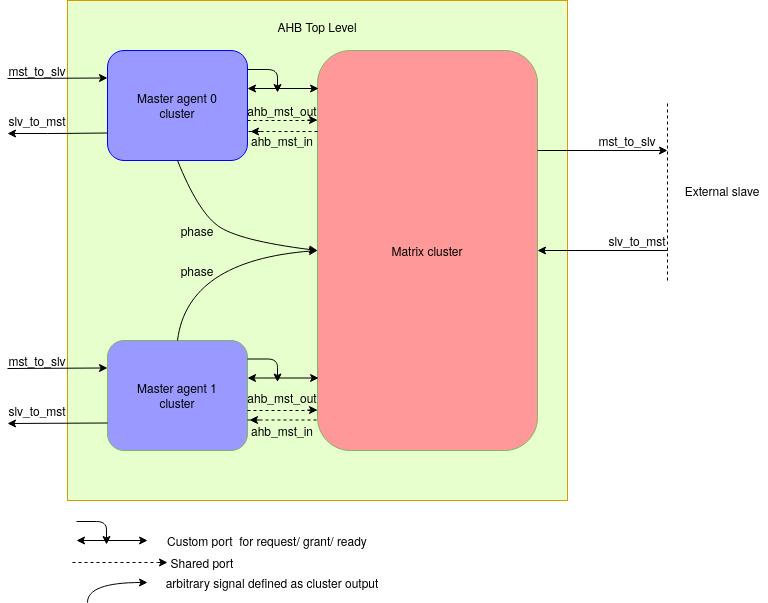
\includegraphics[width=8cm]{figs/Verif/Verif_block.png}
\caption{Verification clusters}\label{fig:verif-clust}
\end{wrapfigure} 

Fig.~\ref{fig:verif-clust} provides an overview of the verification clusters and their connections. I/O connections are listed with their compound names with port type indicated in the legend. The master agent is a relatively simple design so this section is mainly focused on the matrix cluster. The Gap Free Verification process introduced in Sec.~\ref{sub:gfv} is carried out on the matrix cluster. \par
It is not possible to determine every state of the matrix cluster by observing internal registers alone. There are no registers differentiating between a default master being idle or in the data phase of a transfer. Looking at signal values in the past require constraints on wait states. A better alternative is to define the state of the default master agent as an output to its cluster and an input to the matrix cluster. The states are determined based on this signal, address and data bus ownership as well as slave notify signals. \par
The first step is to define a Conceptual State Machine for the matrix cluster and write a set of skeleton properties to cover all core operations. Consider the FSM of the bus matrix from Sec.~\ref{sub:bus-matrix}, where the state \textit{Data} is divided into a set of conceptual states. Each communication over a blocking port signals an important state. The CSM of the matrix cluster, with the required minimum of conceptual states is listed below.    
 
\begin{enumerate}
 \item Idle: No transfer in progress, \textbf{HREADY} is set and bus is ready to accept a new request (1,2).
 \item Address: A transfer is initiated, \textbf{HREADY} is set and bus is ready to accept a new request.(3)
 \item Slave(x)\_write: Important state for each slave output. (4)
 \item Slave(x)\_read: Important state for each slave input (5)
 \item Data\_end: A transfer is completed, \textbf{HREADY} is set and bus is ready to accept a new request. (1,2,3) 
\end{enumerate}

Operation properties must cover all possible requests, read and write transaction to all slaves, success and error response from slaves as well a transaction to the default slave. Most properties have a duration of one time-point, with write transactions, error response from slave and default slave response covering two time-points. \par
The state of the bus is determined by address bus ownership, data bus ownership and which state the default master is in. Address and data bus ownerships are assigned to registers in the arbiter RTL module with the names \textit{master\_sel} and \textit{r\_master\_sel} respectively. The state \textit{Address} can be determined by checking that a single transfer is in progress and it is in the address phase. In the example below, master 0 is the default master. 
\begin{VHI}
macro Address_state : boolean :=
r_master_sel = 0 and agent0 /= data_phase and
(master_sel /= 0 or agent0 = address_phase)
end macro;
\end{VHI}

The state \textit{Data\_end} is determined in a similar fashion, except it is not concerned with any transfer possibly being in the address phase. The next state is decided by checking the address bus if a transfer is in progress and if there are any pending requests.
\begin{VHI}
macro Data_end : boolean :=
(r_master_sel /= 0 or agent0 = data_phase) and hready = true
end macro; 
\end{VHI} 

The only visible registers required to hand over signal values between properties are the signals of the address bus, or more specifically the signals of the address bus which forms part of the payload, including \textbf{HTRANS}. The payload from a granted request is visible on the address bus and \textbf{HTRANS} indicates that a transfer is in progress. \textbf{HWDATA} is fetched directly from the interface of the appropriate agent before the entire payload is assigned the slave outputs. It may appear that \textbf{HWDATA} is sampled in the address phase, but this is corrected in the signal macro using the "next" operator. 
\begin{VHI}
 for timepoints: t_end = t+2; 
 freeze:
   address_bus_haddr_at_t = address_bus_haddr@t,
   agentx_hwdata_at_t = agentx_hwdata@t; --next(agentx_hwdata)
 
 assume:
   at t: Address_state;
   at t: address_bus_haddr = slave0_range;
   at t: address_bus_hwrite = WRITE; 
 
 prove:
   at t_end: slave0_write;
   at t_end: slave0_out_notify = true;
   at t_end: slave0_out_hwdata = agentx_hwdata_at_t;
   at t_end: slave0_out_haddr = address_bus_haddr_at_t;
   during[t+1,t_end]: hready = false; --always determined

\end{VHI}

What remains is to determine the cluster outputs, which are all outputs to the master agents and slaves. All notify signals to the slaves and \textbf{HREADY} must be determined at all times. The remaining outputs should be determined conditionally. No signals on the master agent interface are sampled by the master agent unless \textbf{HREADY} is set. No signals on the slave interface a sampled by the slave unless its accompanying notify is set. \par 
This section has described the essentials for proving completeness on the matrix cluster for single transfers. Extended functionality such as burst transfers are briefly discussed in Sec.~\ref{sec:burst}
 

\section{ESL}
After a complete set of abstract properties for the bus matrix is derived, the ESL model is developed. In the previous section it was established that master agents must be verified in separate clusters. This translates to the ESL by separating the master agents in their own SystemC-PPA module. Defining a suitable interface between the master agent and bus matrix require careful consideration. \par
With blocking ports, correct simulation behavior and the highest level of abstraction is achieved, but that creates an issue with the bus matrix ESL module for multiple masters. Up to three blocking ports need to be serviced in the same time-point due to parallelism, which is not permitted in SystemC-PPA. A helper module is introduced which is not intended for property generation, but to serve as an emulated port interface. The requirements of this module is described in Sec.~\ref{sub:portem}.

\subsection{Bus matrix}
\label{sub:bus-matrix-design}
No more than three explicit states are required to model the bus matrix at the ESL. The implementation of the bus matrix ESL covered in Sec.~\ref{sub:bus-matrix} is elaborated with requirements and options. \par
The communication with the emulated port must occur exactly once in all three states as shown above. It is what signals the conceptual states 1,2 and 5 from Sec.~\ref{sec:bottom-up}. It is required to be a non-blocking write to unconditionally call a wait function, which hands over control to the emulated port so that the requests are updated before they are gotten. 

\begin{C++}
update_requests->try_write(true, sync, "state");  
requests_in->get(reqs); 
\end{C++}


The functionality of the arbitration scheme is carried out in cooperation between the bus matrix and the emulated port. It is essential that the arbitration scheme is modeled equally in the two modules. \par
Fixed-priority arbitration is the scheme chosen for this work, mainly due to its simplicity. It can be modeled with a simple if-else conditional statement that is easily transferable to the emulated port. The "else" clause starting at line 9 in the example below shows the control of the address bus falling back to the default master when no request is pending. 
\begin{C++}
...
else if(reqs.m3_request){
 mAgent_to_bus3->get(payload3);
 AS_regs.haddr = payload3.haddr;
 AS_regs.htrans = NONSEQ;
 AS_regs.hwrite = payload3.hwrite;
 AS_regs.hsize = payload3.hsize;
 addr_owner = 3;
else{
 mAgent_to_bus0->get(payload0);
 AS_regs.haddr = payload0.haddr;
 AS_regs.htrans = NONSEQ;
 AS_regs.hwrite = payload0.hwrite;
 AS_regs.hsize = payload0.hsize;
 addr_owner = 0;
}
\end{C++}

\textit{AS\_regs} only models signals on the address bus and does not include \textit{hwdata}. It is not practical to model \textit{hwdata} in such a way that a visible register mapping is required in the properties. Instead, the bus matrix differentiates read and write transfers when it transitions $Address\rightarrow Data$. Recall from Sec.~\ref{sub:bus-matrix} how the payload data is fetched and subsequently written to the slave. Read transactions must write a zero value to the slave, to avoid the need to account for old values of \textit{hwdata} in each slave. \par
If the slave responds with an error, it is not sufficient to rely on the response payload to relay this information implicitly. The two cycle error response adds an additional cycle, which must be proven in a separate property. Explicitly assigning the error as shown in line 3 below ensures that separate properties are generated for the two different responses, which can be refined accordingly.  
\begin{C++}
slave(x)_to_bus->read(resp, "state");
if(resp.hresp = error){
 to_mAgent(x).hresp = error; //explicitly assign error
}else{
 to_mAgent(x).hresp = resp.hresp; //implicitly assign okay
}
to_mAgent(x).hrdata = resp.hrdata;
to_mAgent(x).hgrant = m(x)_grant;
bus_to_mAgent(x)->set(to_mAgent(x));
} 
       .
       .
update_requests->try_write(true, sync, "data_end");
\end{C++}

The slave response is broadcast to all master agents, which in this work is carried out through shared ports. The slave response can be forwarded through the emulated port, but with almost no return on investment. It is not done in this work to keep the emulated port minimal. The default slave response is given when no slave is selected, which is error status and zero data. \par
Line 8 in the example above shows how \textit{hgrant} is assigned an enum value. The emulated port is not sufficient for representing this signal for multiple master agents and is therefore assigned separately. The value assignement of this signal serve no functional purpose in the ESL model. A boolean value can be assigned if logic is added to set/reset all grants for every possible request.  \par
The transition from the state \textit{Data} is dependent on the address bus and pending requests. The master agent outputs are dependent on which slave is selected. To avoid the need to account for this in the generated properties, default values are assigned before the state transition.   
\begin{C++}
if(AS_regs.htrans == NONSEQ){ 
 nextstate = Data;
 DS_regs = AS_regs;
 //handle requests, update AS_regs accordingly
}else{
 //handle requests, update AS_regs accordingly
 if(request) nextstate = Address;
 else nextstate = Idle;
}
to_mAgent(x).hresp = okay; //assign default values
to_mAgent(x).hrdata = 0;
to_mAgent(x).hgrant = m(x)_grant;
bus_to_mAgent(x)->set(to_mAgent(x));

\end{C++}

 

\subsection{Master Agent}
The SystemC-PPA module of the master agent needs to cover all signals of the master agent interface. Some of these signals are represented in the event handling of the blocking ports. The control flow of a bus request and accompanying signals (\textit{hbusreq, hgrant, hready}) are modeled with a single blocking write as seen from line 3 below. 
\begin{C++}
if(state == request){
  //issue request, wait for grant
  mAgent_request->write(true, "request"); 
  nextstate = address;
}
\end{C++}

The address and control signals are written out on a shared port to be determined in the address phase of the transfer. The blocking write in line 7 models the agent waiting for \textit{hready} to be set. 

\begin{C++}
if(state == address){
  ahb_mst_out.haddr = payload.haddr;
  ahb_mst_out.htrans = NONSEQ
  ahb_mst_out.hwrite = payload.hwrite;
  ahb_mst_out.hsize = payload.hsize;
  mAgent_to_bus->set(ahb_mst_out); //Write address and control to bus
  bus_ready->write(true, "address_phase");
  nextstate = data;
}
\end{C++}

Rather than writing the entire payload to the bus in an instance, the individual payload elements are written in their respective phases both in the ESL and RTL to capture the protocol in operation properties. 

\begin{C++}
if(state == data){
 ahb_mst_out.htrans = Idle; 
 ahb_mst_out.hwdata = payload.hwdata;
 mAgent_to_bus->set(ahb_mst_out); //Write data to bus
 bus_ready->write(true, "data_phase");
 bus_to_mAgent->get(ahb_mst_in); //get response payload
 nextstate = to_master;
}
\end{C++}



 
\subsection{Emulated port}
\label{sub:portem}
The emulated port has strict requirements to ensure correct simulation behavior, both in terms of synchronization and in terms of arbitration. This module can not be proven formally to be a sound abstraction of the RTL for the same reason that it is implemented. The chosen arbitration scheme must be manually verified to exactly match the arbitration scheme in the bus matrix. \par 
\WKSAY{I need to correct where i state that, the bus matrix and the master agent is formally verified, but this interface is verified through simulation on both levels. The starvation plots + assertions show the equality}
\TLSAY{I thought that you verify this by the matrix properties? That's at least what you're stating} 
The port must wait for a synchronization signal from the bus matrix, perform request forwarding, service all applicable blocking ports and return to wait for a synchronization signal without interruption. This is accomplished by utilizing blocking inputs for both ports from each master agent, and performing a non-blocking read, only if there is a writer waiting. 

\begin{C++}
//begin while
update_requests->read(); 
//requests must be reset 
if(mAgent_request->peek()){
mAgent_request->try_read();
requests.mx_request = true;
}
requests_out->set(requests); 
if(bus_ready->peek()) bus_ready->try_read();
//end while
\end{C++}


\section{Refining the Properties}
\label{sec:refine}
This section describes how the generated property sets are refined to hold on the design. Every I/O signal, visible register and important state is represented with a macro, which is of the form 
\begin{VHI}
macro signal_name : type := refinement end macro;
\end{VHI}

The blocking interface in the ESL model has a set of signal macros generated for each port to verify the four phase handshake in the RTL model.
\begin{VHI}
blocking_out_notify : boolean := refinement end macro; --event notify
blocking_out_sync : boolean := refinement end macro;   --wait(event)
blocking_out_sig : type := refinement end macro;       --payload
\end{VHI}


Before covering the individual clusters property refinement, the emulated port interfaces will be explained collectively. \par
\TLSAY{Why would you not first explain the regular clusters and then talk about the complicated emulated port stuff?} 

The emulated port interfaces exclusively use the sync and notify to convey information. Some of these do not exist in the RTL design, so they are given abstract values to satisfy the properties. Following is a pseudo refinement of the existing signals.
\begin{VHI}
--master agent
macro agent0_request_notify : boolean := hbusreq0 end macro;
macro agent0_request_sync : boolean := hgrant0 and hready0 end macro;
macro agent0_ready_sync : boolean := hready0 end macro;

-- bus matrix
macro update_requests_sync : boolean := 
 hbusreq0 or hbusreq1 
end macro;
macro update_requests_notify : boolean :=
 hready0 and hready1 or --example with two masters
 hready0 and hgrant0 or
 hready1 and hgrant1
end macro;
\end{VHI}

The example above show how the connection between the top-level signals is represented on each side of the port. The output in line 2 corresponds with parts of the input in line 8. The output signals from line 11 and 12 correspond to the input signals in line 3 and 4. As long as the logic described in the macros of line 7 and 10 is guaranteed within the emulated port it should not leave a gap in verification. However, this representation is not sufficient to use in the completeness description to determine \textbf{HBUSREQx} as input, or \textbf{HGRANTx} as output. The macros generated from the shared interfaces are used in the completeness description for these two signals in addition. The emulated port interface result in a high number of vacuous properties, up to 45\%. This is due to the conflict between the blocking and shared port, as shown below.
\begin{VHI}
assume:
 at t: not(update_request_sync);
 at t: request  = true;
\end{VHI}

\TLSAY{Where are these two lines of code coming from? You need to put the entire piece of code in it and give it a subtitle. Also in the previous Section you did this see xyz in the two lines below thing. Please find my comment in the previous review on how to deal with code examples.} 

\subsection{Bus Matrix}
All I/O signals of the bus matrix are refined to represent their similarly named top level RTL signal. There are, however, some signals that need some added logic. These are all signals which are represented at the ESL using enum values and signals which are not assigned values on a clock edge in the RTL. \par
One example which cover both scenarios is the signal \textbf{HSIZE} from the master agent. Line 17 shows how the address bus signal is assigned a value from time t, whereas the address bus is actually updated with a signal from time t\_end. Line 1-5 shows how the "next" operator is used on the top-level RTL signal to assign the signal value from the next time-point and how the enum type is accounted for.   
\begin{VHI}
macro agentx_hsize : mask := 
if(next(agentx.hsize) = "000") then MT_B 
elsif(next(agentx.hsize) = "001") then MT_H
else MT_W
end if;
end macro

property request_agentx is
 freeze: 
  agentx_hsize_at_t = agent0_hsize@t;
 
 assume: 
  at t: Idle_state;
  at t: agentx_request;

 prove: 
  at t_end: address_bus_hsize = agentx_hsize_at_t; --t_end = t+1
\end{VHI} 

The output \textit{hgrant} is a similar issue, but in the opposite time direction. It can be determined at t\_end by assigning it the "prev" operator. In this work the choice is instead to assign it an enum value, to avoid unnecessary overhead at the ESL. The enum values \textit{m(x)\_grant} seen in Sec.~\ref{sub:bus-matrix-design} are defined as their own functions in the property set. The default master owns a grant when no other master does and therefore has a separate function. 
\begin{VHI}
macro m(x)_grant : boolean :=
if(agentx_request and not(higher_prio_request) and hready) then true
elsif(addr_own = agentx and not(hready)) then true
else false 
end if;
end macro;
\end{VHI}

The visible registers are the address bus signals and ownership, which are mapped to the physical signals in the arbiter RTL module. The data bus ownership is required to determine some states, but it is removed from the property set through optimaztions done by the tool DeSCAM. Macros for this register and the default master state are added in the refinement process. \par
The state variables from the ESL description are included in the property set although their type and values represent abstract states. A type is added to the RTL signal package, which is never used except to map these state variable to. 


\subsubsection{Completeness Description}
All inputs, as well as the default master state are listed with their signal macro names as determination assumptions. \par
All outputs are listed as determination requirements, most of them conditionally. The unconditional signals are the following: \\

\begin{tabular}{p{4.3cm} | p{10cm}}
\textit{update\_requests\_notify} & Determines \textbf{HREADY} to all master agents. An assertion which proves that they always have the same value is added as dependency. \\
\hline
\textit{bus\_to\_slave(x)\_notify} & Shares the same name as the RTL signal \\
\textit{slave\_to\_bus(x)\_notify} &  \\
\end{tabular}

The top two signals are used as conditions to determine the remaining outputs. The slave outputs are determined if \textit{bus\_to\_slave(x)\_notify} is set and \textbf{HRDATA}, \textbf{RESP} and \textbf{HGRANTx} are determined if \textit{update\_requests\_notify} is set. \par

The visible registers for the address bus and address bus ownership are listed as local determination requirements. The data bus ownership is not listed here, because it is optimized away from the property set. It is not used to directly determine any outputs so it can be left out without failing any determination checks, although it would ideally be covered by the property set as an added precaution. \par
Finally, in the case of a single master system, an assertion is added to prove that requests can only occur if the master agent is in the corresponding state. This assertion is added to the dependencies of the completeness description so that the case split test holds. 

\subsection{Master Agent}
The property set and completeness description is identical for all master agents, therefore it is only refined for one master. 
All I/O signals except the emulated port interfaces are refined with their similarly named top-level RTL signal. In the master agent, \textit{hsize} is an output, so therefore determining the the signal as seen in the previous section, an assertion is added to prove this correspondence. \par
The registers storing the requests are refined to mAgent0/(xx)\_reg. All states are refined to the corresponding state of the RTL design.\par
The completeness description lists all inputs and outputs with the signal macros generated from the SystemC-PPA. The emulated port interfaces are sufficient to determine all signals used within the macros. The state of the agent is added as a determination requirement so that it can be used as an input to the matrix cluster.  

\section{RTL}
The open source architecture used in this work is defined in one architectural module; \textit{ahb\_arbiter.vhd}. It uses arbitration functions from the file \textit{ahb\_func.vhd}, slave address configurations from \textit{ahb\_configure.vhdl}, packages from \textit{ahb\_package.vhd} and components from \textit{ahb\_component.vhdl}. \par
All payloads and state machine declarations used in the agents are added to the package file, as well as the unused type representing the ESL states of the bus matrix. It also contains some constants to offer readability for the signals which are hardwired. \par
Component declaration of all system modules are added to the component file, this includes agents, arbiter and bus matrix. The bus matrix is a top-level module for the arbiter, which instantiates the arbiter and provides default master selection and master priority. Master zero is highest priority, with priority decreasing with incrementing numbers. For simplicity, the highest priority master is set as the default in this work. \par
The configuration file contains the slave address ranges in decimal number, as well as the remapped address ranges of the slaves. Remap is not implemented in this work so they must be equal, remap is hardwired to zero for extra security. \par
The top-level module must include the following: \textit{library ieee}, \textit{logic\_1164} and \textit{numeric\_std} from ieee, \textit{ahb\_package} and \textit{ahb\_components}. \par
The arbiters reset is active low, so the top-level reset must be inverted before assigning it to the matrix port map. All slave agents require their address offset as a generic in the form of a 32-bit logic vector. All master and slave agents are connected to their inputs and outputs of the matrix with corresponding numbers. 

\subsection{Slave Agent}
The slave agent includes the same packages as the top-level, except for the components. It includes an additional package \textit{std\_logic\_unsigned} so that the slave address offset can be subtracted from the haddr input. \par
\begin{wrapfigure}[12]{l}{6cm}
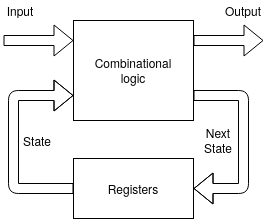
\includegraphics[width=5cm]{figs/hw/statemachine.png}
\caption{State machine}\label{fig:statem}
\end{wrapfigure} 

The slave agent is implemented as a state machine where combinational logic decide the next state based on internal registers and inputs. The state transitions are covered in Sec.~\ref{sub:sagent} and will not be reiterated here. What is covered is how the output assignments are handled so that properties can be generated from an ESL description which can be refined to hold on the design. These outputs are the request and response payload signals. \par
The request payload is stored in output registers after they are sampled in the address phase. When the signals are stored, the address offset is subtracted from \textbf{HADDR} and \textbf{HWDATA} is zeroed. If it is a write transaction, \textbf{HWDATA} is overwritten with the data bus value on the following cycle. \par
The response payload is stored in response registers and a flag is set simultaneously. The slave agent waits for \textbf{HREADY} to be set and zeroes the response payload registers.  



\subsection{Master Agent}
The master agent uses the same type of state machine as the slave agent. The functionality of the master agent is mirrored in the ESL description. Flags are set before the transfer phases are inititated, which signal when the address, control and data is written to the bus. 


\section{Building the Generator}
The generator consists of two parts; the hardware generator and the plugin which generates and refines the property sets. The hardware generator takes number of masters and slaves as input arguments. It begins by checking that the input arguments are within the range 1-15 and reads a text file containing slave address ranges. The slave address ranges are stored in a map. The generator instantiates two classes with this data which generate the system at the RTL and ESL. The generator produces a text file with the same stored data, converted for use within the plugin. It continues to call the plugin with the bus matrix and master agent SystemC-PPAs in turn. The plugin reads the text file and distinguishes between the two SystemC-PPAs to generate a refined property set and completeness description for each. 

\subsection{Hardware generator}
The generator uses the slave input argument to decide how many lines of the address map text file to read. It recognizes the words "start" and "end" to determine the start and end of the range. A separate map is produced for the ESL and RTL generation to avoid the need to convert the address format on the fly. The classes which generate the ESL and RTL are so similar in structure and function that they will not be described separately. \par
A set of files are generated for each abstraction layer, which are files that are not static with respect to number of masters and slaves. All files such as agents, dummies for test bench and arbiter remain in the output folder untouched and must not be deleted or modified. \par
All files are generated with an output file stream which is assigned a function output. Each file has its own dedicated function which write the module description to a local string stream. Each function uses the stored number of masters, slaves and address map to produce its module according to the requested configuration. 

\subsection{Plugin: PrintAHB}
The plugin starts by reading the plugin data text file, which contain number of masters and slaves, as well as slave address ranges. The slave address ranges were used in an earlier implementation, but are not removed from the plugin data in case they are needed in the future. The plugin checks the file name if it is the bus matrix or master agent and calls the appropriate function to generate the property files. \par
DeSCAM creates an abstract model of the SystemC-PPA which is stored in a C++ object. This object contains maps and objects which together store all I/O signals, all variables, the FSM, property-suite etc. The plugin iterates over the components of the abstract model to simultaneously generate and refine the property macros as well as property set and completeness description.

\subsubsection{Bus matrix}
The I/O signals of the ESL design and RTL are given the same names, which simplify the automatic property refinement. The plugin iterates over a port map, converts the abstract signal name to its corresponding RTL signal name and writes it to a string stream. The process is shown in the following example.
\begin{C++}
stringstream ss;
for(auto dp: ps->getDpSignals)
 //iterates over I/O signals in the abstract model
 ss << "macro" << dp->getName(); // insert name
 ss << //insert datatype

 ss << dp->getName().substr(0, dp->getName().find("_sig"));
 //Signals share name up to the "_sig" component added by the tool

 ss << "end macro"; 
 }
\end{C++}



Some signals require more elaborate refinements, as is covered in Sec.~\ref{sec:refine}. These signals are checked for with if-else statements and refined accordingly when found. \par
The required assertions and macro functions are added for the appropriate number of masters. The macros for data bus ownership and default master state are subsequently added. The visible registers do not share signal names with the RTL design, so every one is checked for by name and refined accordingly. \par

\TLSAY{This reads like a list. Why not having it as a list?} 
The states are given recognizable names and numbering in the ESL model, which are transferred to the abstract model but with added numbering. The plugin iterates over the state map and refines the state macro according to name. If the state contains important numbering, this number is fetched with a function that excludes the numbering added by the tool. \par
Each operation property is generated using functions which are slightly modified versions of functions from the plugin \textit{PrintITL} from \cite{descam}. Mainly, it modifies the time-points in the properties which require two cycles to complete by checking the assumptions and commitments. The generator excludes vacuous properties from generation. This is accomplished by checking for conflicts in the assumption part of each property. Some of these conflicts lead to conflicts in the completeness check, so they must be removed. The number of vacuous and non-vacuous properties are displayed on the terminal. 
\par
Generating systems with one or two masters lead to additional vacuous properties which are not removed. These properties cover transitions which only could occur if more master were connected. They are, however, required to remain to satisfy the case split test. Added assertions can replace the vacuous properties, although they are not yet discovered. 

\subsubsection{Master agent}
The master agent is refined to hold on master agent zero in a similar, but simpler manner than the bus matrix. There are no vacuous properties which need to be removed. 



\section{Simulation}
\label{sec:sim}
Corresponding simulation models are generated for the RTL and ESL model. The simulation models offer a second layer of verification that the operations are carried out as intended and that the architecture behave equally at both levels. \par
Master and slave dummies which carry out simple read and write operations are connected to the top-level design. The slave dummy has no knowledge of its address offset, or which master is operating it. Similarly, the master can not distinguish if the slave it intended to access is the slave which is responding. VHDL does not offer the same high level capabilities as C++, but the simulation models should operate on equal principles. This is accomplished by adding an identification number as input to the slave dummies in the RTL model and global functions to encode and decode identification numbers in both models. 
\TLSAY{Now there are dummies. another picture would be nice. It's confusing.} 

\begin{itemize}
 \item \textit{Write}: The master dummy calls a function from the included \textit{globals.h/.vhdl}, which takes target address as input argument and returns an ID number. The master adds this ID number to the top eight bits of its payload data. The slave dummy asserts that the top eight bits of the received data matches its own ID number. The ESL slave dummy must translate its object name to the corresponding ID number with a function available in the same included file. 
 \item \textit{Read}: The slave dummy adds its ID number to the top eight bits of its response data. The master dummy uses a function to assert that the response ID matches its target address ID.   
\end{itemize}  

It is highly unlikely that errors in the global functions correspond to errors in the design, or in other words masks them. \TLSAY{Can it happen or can it not happen? If it can happen, explain what kind of errors are missed. If it can't happen remove it} The simulations are run for $10^6$ transfers, which are counted within the slave dummies, out of range transfers are therefore not counted and affects simulation time.  

\subsection{Starvation}
One drawback of fixed-priority arbitration is that lower priority masters may never be granted access to the bus. When this occurs depend on the amount of masters, the rate of transfer for each master and the duration of each transfer. The plot below show\TLINS{s} when the masters are granted access to the bus, based on the duration and transfer rate in the RTL model. The different transfer durations are separated for each run to get comprehensive results and the slave dummies respond without delay. The plot shows a clear separation and linear relationship between the different transfer conditions and rates. 
\TLSAY{This section is very confusing. Did you explain it somewhere? Why is read succsess/write fail intermixed? Is this an RTL or ESL simulation. If it is an ESL simulation why is there a clock delay? If this is an RTL simulation where is the ESL counterpart ? Professors will jump on this, because your fiddeling with the asynchronous model here. Make it crisp} 
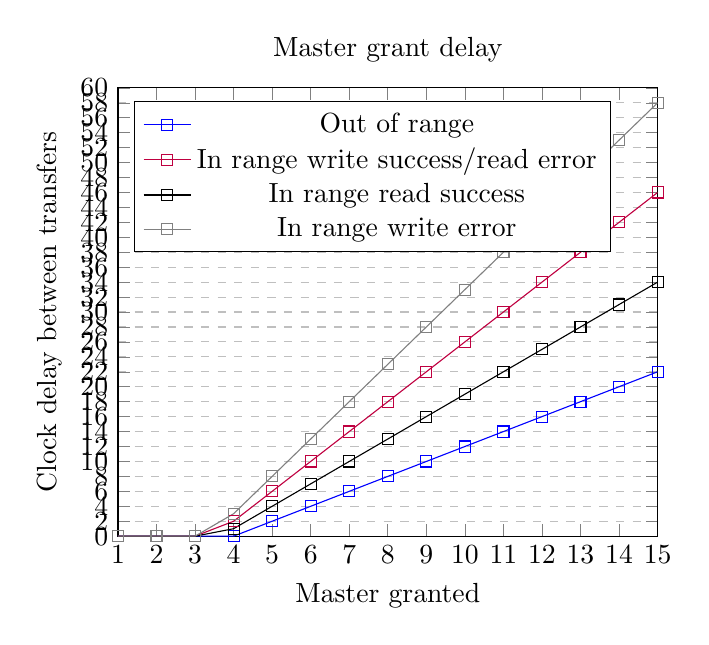
\begin{tikzpicture}
\begin{axis}[
    title={Master grant delay},
    xlabel={Master granted},
    ylabel={Clock delay between transfers},
    xmin=1, xmax=15,
    ymin=0, ymax=60,
    xtick={1,2,3,4,5,6,7,8,9,10,11,12,13,14,15},
    ytick={0,2,4,6,8,10,12,14,16,18,20,22,24,26,28,30,32,34,36,38,40,42,44,46,48,50,52,54,56,58,60},
    legend pos=north west,
    ymajorgrids=true,
    grid style=dashed,
]
\addplot[
    color=blue,
    mark=square,
    ]
    coordinates {
    (1,0)(2,0)(3,0)(4,0)(5,2)(6,4)(7,6)(8,8)(9,10)(10,12)(11,14)(12,16)(13,18)(14,20)(15,22)

    };
    \addlegendentry{Out of range}

\addplot[
    color=purple,
    mark=square,
    ]
    coordinates {
    (1,0)(2,0)(3,0)(4,2)(5,6)(6,10)(7,14)(8,18)(9,22)(10,26)(11,30)(12,34)(13,38)(14,42)(15,46)

    };
    \addlegendentry{In range write success/read error}

\addplot[
    color=black,
    mark=square,
    ]
    coordinates {
    (1,0)(2,0)(3,0)(4,1)(5,4)(6,7)(7,10)(8,13)(9,16)(10,19)(11,22)(12,25)(13,28)(14,31)(15,34)
    };
    \addlegendentry{In range read success}

\addplot[
    color=gray,
    mark=square,
    ]
    coordinates {
    (1,0)(2,0)(3,0)(4,3)(5,8)(6,13)(7,18)(8,23)(9,28)(10,33)(11,38)(12,43)(13,48)(14,53)(15,58)

    };
    \addlegendentry{In range write error}

\end{axis}
\end{tikzpicture}


\TLSAY{Here comes the ESL model ... okay ... this section needs more structure. Why don't start at the ESL and go down? ... I think you should explain the setup better.  This 0ps and 1ps is also very confusing. Why don't you explain two modes? One using SC\_ZERO\_TIME the other one uses 1ps (Which models are random selection of the next operation) ... you should also explain what your setup looks like}

\TLSAY{I had the impression that you explained to me that the wait of the dummies random ? So you would use mod WAITCOUNT ... in case of rnd() mod 5 the master may wait 0,1,2,3,5 steps? Here you claim that you're waiting exactly 1,2,3,4,5 } 



The ESL model has no notion of time, which entails that the modeling of starvation is not inherently equal to the RTL. Because it is an untimed model, the y-axis of the plot below is not delay in time, rather it is the amount of wait functions called. \par
The bus matrix at the ESL differentiate between read, write and error without interrupting, or otherwise delaying the completion of the transaction. The bus matrix does differentiate between in and out of range transfers, in a similar manner to the RTL model, provided that the wait function is called with a non-zero wait time. 
The plot shows how a global wait time of zero incur a non-linear relationship between the amount of wait functions and starvation for out of range transfers.

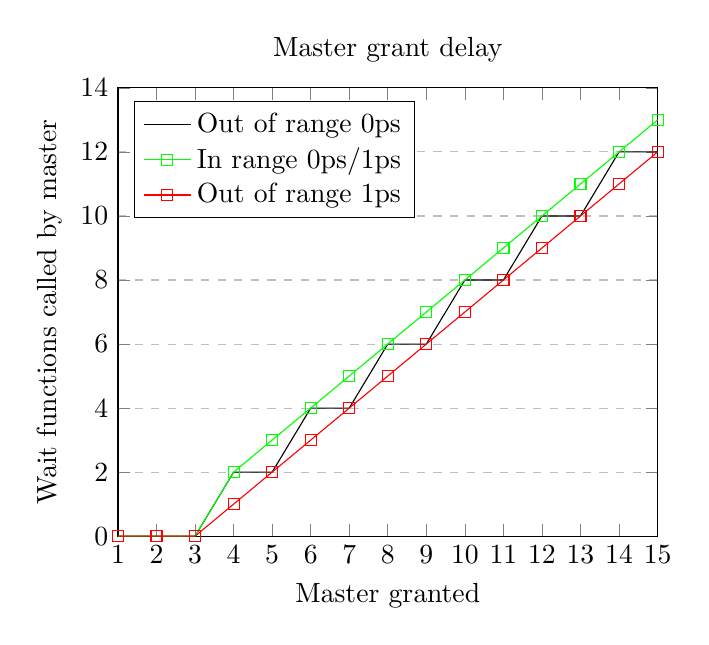
\begin{tikzpicture}
\begin{axis}[
    title={Master grant delay},
    xlabel={Master granted},
    ylabel={Wait functions called by master},
    xmin=1, xmax=15,
    ymin=0, ymax=14,
    xtick={1,2,3,4,5,6,7,8,9,10,11,12,13,14,15},
    ytick={0,2,4,6,8,10,12,14},
    legend pos=north west,
    ymajorgrids=true,
    grid style=dashed,
]

\addplot[ 
  color=black,
    mark=circle,
    ]
    coordinates {
    (1,0)(2,0)(3,0)(4,2)(5,2)(6,4)(7,4)(8,6)(9,6)(10,8)(11,8)(12,10)(13,10)(14,12)(15,12)

    };
    \addlegendentry{Out of range 0ps}

\addplot[
   color=green,
    mark=square,
    ]
    coordinates {
    (1,0)(2,0)(3,0)(4,2)(5,3)(6,4)(7,5)(8,6)(9,7)(10,8)(11,9)(12,10)(13,11)(14,12)(15,13)

    };
    \addlegendentry{In range 0ps/1ps}

\addplot[
   color=red,
    mark=square,
    ]
    coordinates {
    (1,0)(2,0)(3,0)(4,1)(5,2)(6,3)(7,4)(8,5)(9,6)(10,7)(11,8)(12,9)(13,10)(14,11)(15,12)

    };
    \addlegendentry{Out of range 1ps}



\end{axis}
\end{tikzpicture}

It is feasible to implement a monitor which keeps track of transactions and notifies if a master is granted the bus when it should starve and vice versa. It keeps track of transfer direction, success and context switching. How the monitor can accurately calculate when each master will starve, without using cycle accurate timing is not know and beyond the scope of this work. It is, however, possible to use this data to design a monitor which under-approximates when a master is granted the bus. If the simulation does not indicate that any masters connected to the system starves forever, the system is safe to implement at the RTL. If the over-approximation indicates that a master will starve, an alternative configuration or arbitration scheme should be considered. 


\TLSAY{You have it a little in your wrap up, but why is this simulation necessary? What kind of results do we expect to get. Why is is not 1:1 transferable. What does this mean for soundness? This section feels really rough.}  


\section{Experimental Results}

\TLSAY{This section is not done yet right? Where are the result for ESL simualtion. Where is the comparsion ESL/RTL? Where is you discussion of the results} 
Comparisons are made between the RTL model and its PPA representation, to determine the effica\TLINS{n}cy of the abstraction. Table \ref{tab:stats} compare the resource demand of the different models with respect to configuration size. The variables listed in the PPA section are variables available in the abstract model and does not count intermediate variables used in the ESL model. One additional input and visible register are added to the property set during the refinement process, which are not listed in the table. The total resources for the bus matrix is the sum of the three bottom rows.

\begin{table}[hbt] 
  \begin{tabular}{ l r r r r r}
  \hline 
  \hline
      & \multicolumn{2}{c}{\textbf{\_\_\_}RTL\textbf{\_\_\_}} & \multicolumn{3}{c}{\textbf{\_\_\_\_\_\_}PPA\textbf{\_\_\_\_\_\_}} \\
  Modules & inp./out. & FFs & inp./out & var. & states \\
    \hline
  Master agent & 107/114 & 175 & 2/4 & 12 & 5 \\
  \hline
  Bus matrix & - & 114 & 1/1 & 5 & 3 \\
  
  Per slave & 107/114 & 193 & 1/1 & - & 2 \\
 
  Per master & 106/47 & 111 & 1/1 & - & - \\
    \hline
    \hline  
  \end{tabular}
\caption{AHB resource comparison}
\label{tab:stats}
\end{table}

The simulation models introduced in Sec.~\ref{sec:sim} were run on a range of configurations. The efficiency of simulating at the ESL compared to the RTL is clear. The simulations ran for a total of $10^6$ transactions, independent of configuration size, where the ESL simulation time was 7-8 seconds in all cases, with the variation occurring for different runs on the same configuration. The RTL simulation times are shown in the figure below. All simulations were run on the same computer on the same day. The ESL models were built and run with cmake3, whereas the RTL models were built and run with Modelsim SE-64 10.7c. All RTL simulations were run without displaying signals as waveforms. \\
\WKSAY{These simulations are run locally at uni because frascati was to variable and kept disconnecting. What is interesting is that on frascati, the ESL simulations are faster (6-7s) and RTL simulations are slower, with almost a minute in difference in some cases}

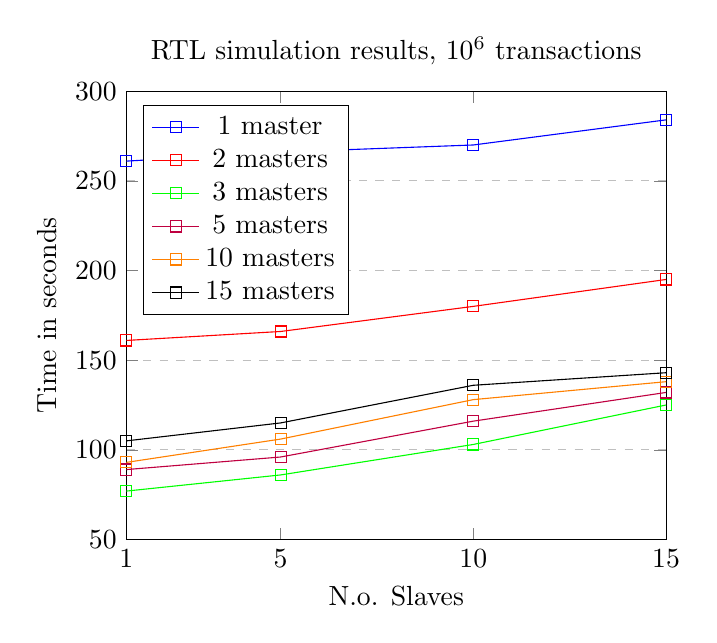
\begin{tikzpicture}
\begin{axis}[
    title={RTL simulation results, $10^6$ transactions},
    xlabel={N.o. Slaves},
    ylabel={Time in seconds},
    xmin=1, xmax=15,
    ymin=50, ymax=300,
    xtick={1,5,10,15},
    ytick={50,100,150,200,250,300},
    legend pos=north west,
    ymajorgrids=true,
    grid style=dashed,
]
\addplot[
    color=blue,
    mark=square,
    ]
    coordinates {
    (1,261)(5,266)(10,270)(15,284)

    };
    \addlegendentry{1 master}

\addplot[
    color=red,
    mark=square,
    ]
    coordinates {
    (1,161)(5,166)(10,180)(15,195)
    };
    \addlegendentry{2 masters}

\addplot[
    color=green,
    mark=square,
    ]
    coordinates {
    (1,77)(5,86)(10,103)(15,125)
    };
    \addlegendentry{3 masters}

\addplot[
    color=purple,
    mark=square,
    ]
    coordinates {
   (1,89)(5,96)(10,116)(15,132)
    };
    \addlegendentry{5 masters}

\addplot[
    color=orange,
    mark=square,
    ]
    coordinates {
    (1,93)(5,106)(10,128)(15,138)
    };
    \addlegendentry{10 masters}

\addplot[
    color=black,
    mark=square,
    ]
    coordinates {
    (1,105)(5,115)(10,136)(15,143)
    };
    \addlegendentry{15 masters}
    
\end{axis}
\end{tikzpicture}

The simulation time of configurations with one and two masters are offset due to the delay between transfers. It is not the simulation itself that is less efficient, it is the system that require more cycles to complete the transfers. This latency is induced by a lack of parallelism within the master agent. \par

The amount of generated properties depend on amount of masters and slaves connected to the system. The figure below show the relationship between properties and configuration sizes. Vacuous properties are not counted. The proof time of each properties varies between 1-10 seconds for the small configurations up to 1-2 minutes for the largest.

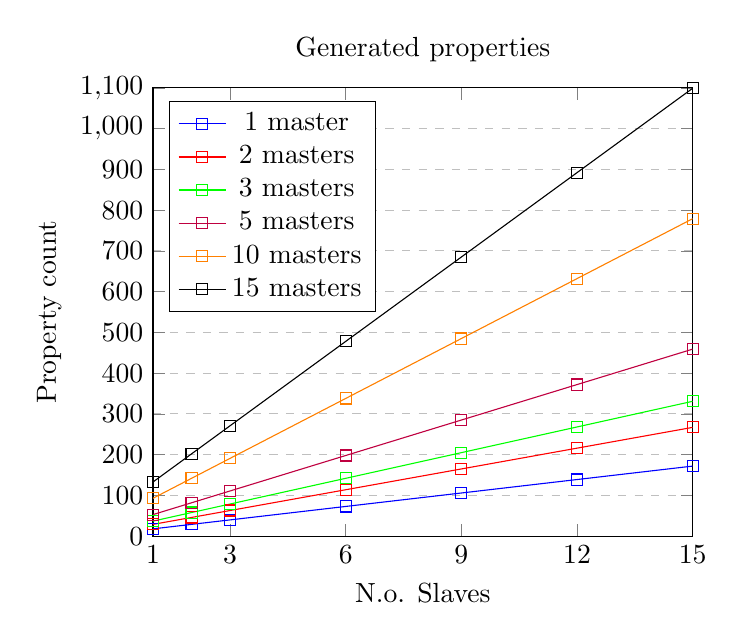
\begin{tikzpicture}
\begin{axis}[
    title={Generated properties},
    xlabel={N.o. Slaves},
    ylabel={Property count},
    xmin=1, xmax=15,
    ymin=0, ymax=1100,
    xtick={1,3,6,9,12,15},
    ytick={0,100,200,300,400,500,600,700, 800, 900, 1000, 1100},
    legend pos=north west,
    ymajorgrids=true,
    grid style=dashed,
]
\addplot[
    color=blue,
    mark=square,
    ]
    coordinates {
    (1,18)(2,29)(3,40)(6,73)(9,106)(12,139)(15,172)

    };
    \addlegendentry{1 master}

\addplot[
    color=red,
    mark=square,
    ]
    coordinates {
    (1,29)(2,46)(3,63)(6,114)(9,165)(12,216)(15,267)
    };
    \addlegendentry{2 masters}

\addplot[
    color=green,
    mark=square,
    ]
    coordinates {
    (1,37)(2,58)(3,79)(6,142)(9,205)(12,268)(15,331)
    };
    \addlegendentry{3 masters}

\addplot[
    color=purple,
    mark=square,
    ]
    coordinates {
   (1,53)(2,82)(3,111)(6,198)(9,285)(12,372)(15,459)
    };
    \addlegendentry{5 masters}

\addplot[
    color=orange,
    mark=square,
    ]
    coordinates {
    (1,93)(2,142)(3,191)(6,338)(9,485)(12,632)(15,779)
    };
    \addlegendentry{10 masters}

\addplot[
    color=black,
    mark=square,
    ]
    coordinates {
    (1,133)(2,202)(3,271)(6,478)(9,685)(12,892)(15,1099)
    };
    \addlegendentry{15 masters}
    
\end{axis}
\end{tikzpicture}




\section{Concept: Burst Transfers}
\label{sec:burst}
